\documentclass[aspectratio=43, a4paper, 12pt]{beamer}

% Packages
\usepackage{animate}
\usepackage{graphicx}
\usepackage{multicol}
\usepackage{charter}

% Language
\usepackage[utf8]{inputenc}
\usepackage[T1]{fontenc}
\usepackage{babel}


% Beamer
\usetheme{Singapore}
\usecolortheme{default}

\setbeamertemplate{items}[ball]
\setbeamertemplate{section in toc}[ball]
\setbeamertemplate{subsection in toc}[ball]
\setbeamercolor{section number projected}{bg=gray,fg=white}
\setbeamercolor{subsection number projected}{bg=gray, fg=white}
\setbeamercolor{item}{fg=gray}
\setbeamercolor{navigation symbols}{fg=black}
\addtobeamertemplate{background canvas}{\transfade[duration=0.2]}{}

\setbeamertemplate{navigation symbols}{}

\AtBeginSection[]
{
  \begin{frame}<beamer>
    \tableofcontents[currentsection]
  \end{frame}
}


% Footline
\definecolor{author_bg}{RGB}{204, 204, 236}
\setbeamercolor*{author_foot}{bg=author_bg, fg=black}
\setbeamercolor*{title_foot}{parent=palette secondary}

\setbeamertemplate{footline}
{	
	\hbox{
	 	\begin{beamercolorbox}[wd=0.5\paperwidth, ht=2.25ex, dp=1ex, right]{title_foot}
			\insertshorttitle \hspace{1em} 
		\end{beamercolorbox}%
		
	 	\begin{beamercolorbox}[wd=0.4\paperwidth, ht=2.25ex, dp=1ex, left]{author_foot}
		   	\hspace{1em} \insertshortauthor
	  	\end{beamercolorbox}%
	  	
	  	\begin{beamercolorbox}[wd=0.1\paperwidth, ht=2.25ex, dp=1ex, left]{author_foot}
		   	\hspace{1em} \insertframenumber~|\ \inserttotalframenumber
	  	\end{beamercolorbox}%	  	 
	}
}


\title{Projet numérique~: Soutenance finale}
\subtitle{Modèle de Vicsek}
\author{ROYER Antoine and PEYROUTET Alexis}
\institute{L3 PCAME – Tarbes}
\date{}

\begin{document}
	\begin{frame}
		\titlepage
		
\includegraphics[width=3cm]{images/ut3.png} \hfill 
\includegraphics[width=2.5cm]{images/uppa.png}
	\end{frame}
	
\section{Présentation et explication}
\subsection{Présentation du modèle}
\begin{frame}{Présentation du modèle}
		\begin{columns}
			\begin{column}{0.5\paperwidth}
			\only<1>{\begin{center} 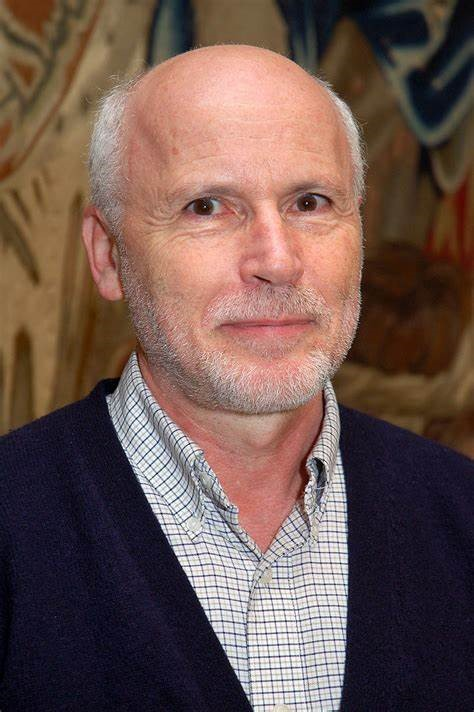
\includegraphics[width=4cm]{images/photo_vicsek.jpg}  \end{center}}
			\only<2>{\begin{center} 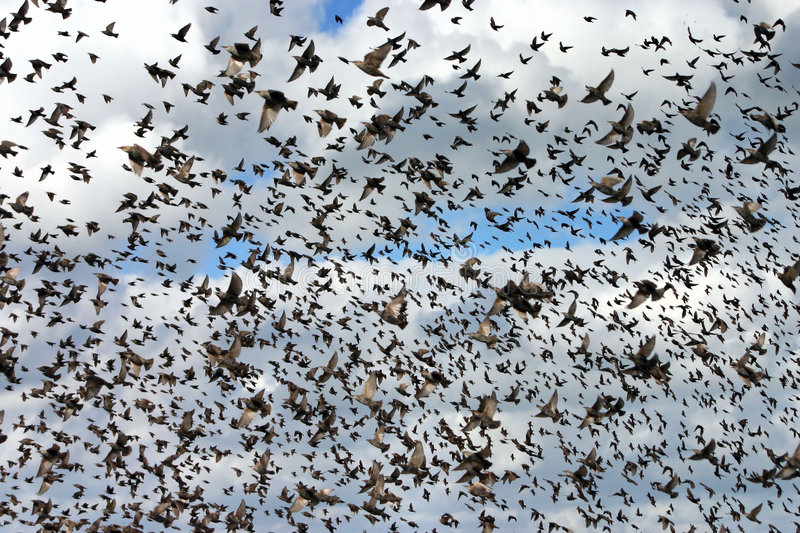
\includegraphics[width=6cm]{images/essaim_oiseau.jpg} \\ Essaim d'oiseaux \end{center}}
			\only<3>{\begin{center} 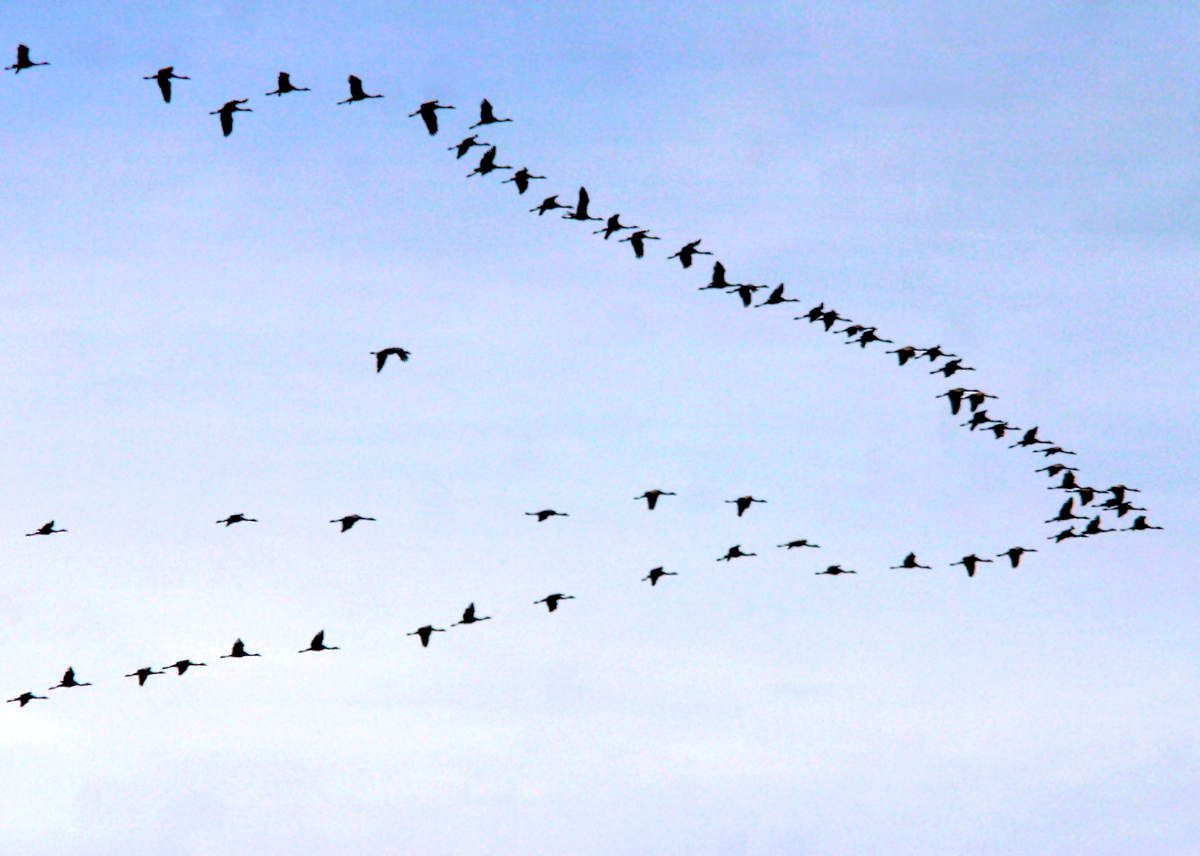
\includegraphics[width=6cm]{images/grues.jpg} \\ Migration des grues \end{center}}
			
			\only<4>{\begin{center} 
\includegraphics[width=6cm]{images/calendrier.jpg} \end{center}}
			\end{column}
			
			\begin{column}{0.5\paperwidth}
				\begin{itemize}
					\item<1-> Tamás \textsc{Vicsek} (74 ans)~;
					\item<2-> Etude des mouvements collectifs (systèmes auto-organisés)~;
					\item<3-> Auncun agent leader dans le modèle~;
					\item<4-> Création du modèle en 1995.
				\end{itemize}			
			\end{column}
		\end{columns}		
	\end{frame}
	
\subsection{Explications sur le modèle}

\begin{frame}{Les bases du modèles}

\only<1>{\begin{center}Le modèle de \textsc{Vicsek} permet d'étudier un groupe d'agents qui se déplace dans un espace.\end{center}}
\only<1>{\begin{center} 
\includegraphics[width=4cm]{images/regle.jpg}  \end{center}}

\only<2>{\begin{center}Chacun des agents a une vitesse donnée (~en norme et en direction~) et va interagir avec ses voisins.\end{center}}
\only<2>{\begin{center} 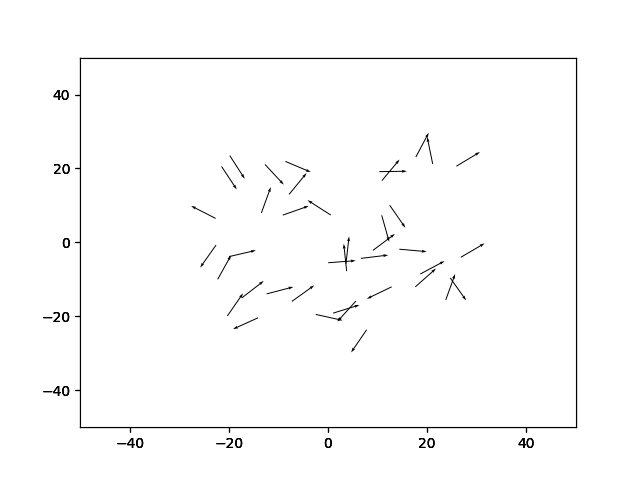
\includegraphics[width=8cm]{images/image_3.png}  \end{center}}

\only<3>{\begin{center}Création d'un mouvement de groupe suite aux interactions entre les agents.\end{center}}
\only<3>{\begin{center} 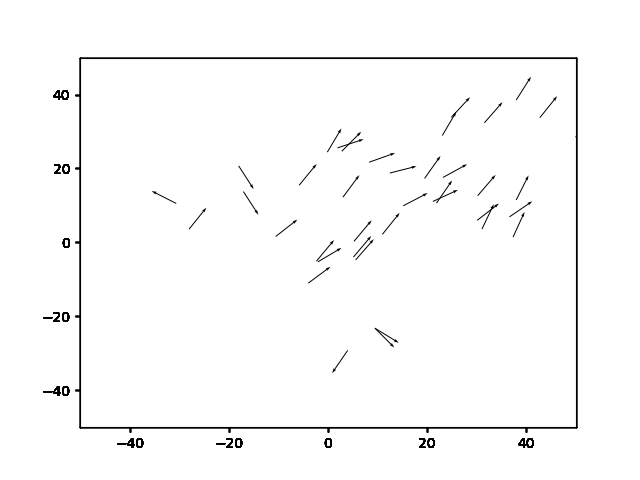
\includegraphics[width=8cm]{images/image_4.png}  \end{center}}

\end{frame}

\begin{frame}{Les équations du modèle}

		\only<1-3>{\begin{center} \[ \left\{ \begin{array}{rcl}
		\Theta_{i}(t + \text dt) & = & \Theta_{j |r_{i}-r_{j}|<r} + \eta_{i}(t) \\[0.2cm]
		r_{i}(t + \text dt) & = & r_{i}(t) + v_{i}\Delta t
	\end{array} \right. \]  \end{center}} 
		\begin{itemize}
				   \item<1-3> $r_{i}$ la position de chaque individu~;
				   \item<2-3> $i$ est l'indice de l'agent en question et $t$ le temps.~;
					\item<3-3> $\eta$ le bruit et $\Theta$ l’angle définissant la direction de sa vitesse~;
		\end{itemize}
				
		\vspace{-2cm}\only<4-5>{\begin{center} \[ \left\{ \begin{array}{rcl}
		\Theta_{i}(t + \text dt) & = & \Theta_{j |r_{i}-r_{j}|<r} + \eta_{i}(t) \\[0.2cm]
		r_{i}(t + \text dt) & = & r_{i}(t) + v_{i}\Delta t
	\end{array} \right. \]  \end{center}} 
		\begin{itemize}
				   \item<4-> $\Theta_{j |r_{i}-r_{j}|<r}$ est la direction moyenne des vitesses des agents dans un cercle de rayon $r$~;
					\item<5->  $j$ représentera alors l'ensemble des voisins de $i$ compris dans ce cercle.		
					
		\end{itemize}
	\end{frame}
	
\begin{frame}{Autres intérêts du modèle}
\only<1>{\begin{center}Comportement des foules et construction de bâtiments\end{center}}
\only<1>{\begin{center} 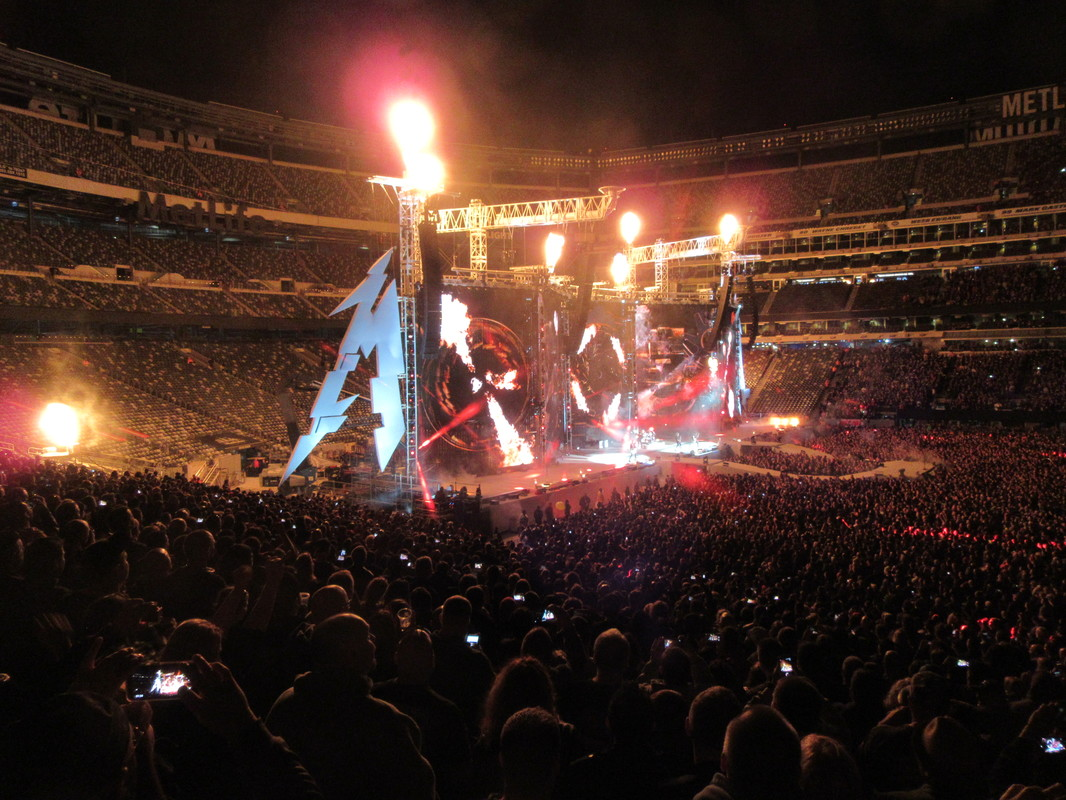
\includegraphics[width=8cm]{images/foule.jpg}  \end{center}}

\only<2>{\begin{center} Domaine de la robotique\end{center}}
\only<2>{\begin{center} 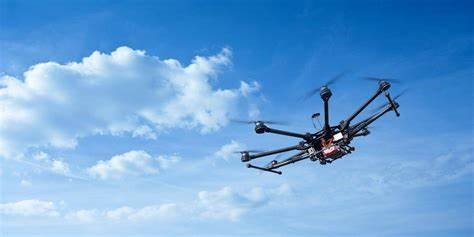
\includegraphics[width=8cm]{images/drone.jpg}  \end{center}}

\end{frame}

\section{Méthode utilisée}

\end{document}



